%*****************************************
\chapter{Background}
\label{ch:background}
%*****************************************
%\hint{This chapter should give a comprehensive overview on the background necessary to understand the thesis.
%The chapter should have a length of about five pages!}

To develop this work a common base of concepts is needed. This chapter aims to establish the fundamental ideas necessary to comprehend this thesis.\\
%As such a recap can never be totally comprehensive prerequisites are %unavoidable. 
%The most notable are:
%\begin{itemize}
	%\item Understanding the concept of over-fitting
	%\item ...
%\end{itemize}

\section{Neural Networks}
\subsection{Basics}
Neural networks are a part of most major AI-breakthrough in the last decade enabling computers to compete in fields formerly championed by humans.\footnote{\begin{itemize}
		\item 
			2011: "Watson" of IBM defeats two former grand champions in "Jeopardy!" \cite{lally2011natural}
		\item 
			2011: "Siri" enables users to use natural language to interact with their phones 
			\cite{ARON201124}
		\item 
			2015: A convolutional neural network classifies images from the ImageNet dataset more accurately than human experts 
			\cite{Russakovsky2015} \cite{He_2015_ICCV}
		\item 
			2016: "AlphaGo" beats Lee Sedol, one of the world's strongest Go players
			\cite{gibney2016google} \cite{silver2017mastering}
	\end{itemize}
}
They implement a statistical understanding of AI, which is to say that they try to find a specific model optimizing the likelihood of reproducing input-output pairs similar to some training data. The competing philosophy directly divines behaviour rules, frequently from expert knowledge, and as such is far less dependant from data.  
\textcolor{red}{[citation needed]}\\
For the former concept its model classes are the essential point of design. A multitude of properties maybe sought after in a model class of which a few important ones are:
\begin{itemize}
	\item \textbf{Richness:}\\
	The diversity of single models in the class and thus the ability to fit a wide field of different input-output landscapes.\footnote{
		More formally the richness of a model class can be described as the amount of different functions from the input-space to the output-space which can be expressed through a model of said class.}\\
	If a model class is inherently restricted the underlying relation between inputs and outputs might simply be beyond the expressive capabilities of all its models.\\
	In other words: If a model class is not rich enough all of its models will underfit the given training data.
	\item \textbf{Stability:}\\ 
	Tendency of similar models in the class to handle inputs in a similar way.\\
	If your model class shows unstable behavior defining a sensible way to search it for good models becomes difficult.
	\item \textbf{Interpretability of Models:}\\
	 Ease of formulating knowledge out of any given model in the class.\\
	 As fields exist in which statistical AI outperform experts the extraction of knowledge understandable and applicable by humans is of special interest.
	\item \textcolor{red}
	{[citation needed]}
\end{itemize}
If one knows an entity that already performs well on a given task it is a sensible approach to design ones model class to reproduce its decision process. Humans usually are such entities for many tasks of interest to AI research so they are a natural source of inspiration. Neural networks essentially are simplified models of a human central nervous system. \\
The most basic building block of the human central nervous system is a neuron which can receive multiple stimuli and is able to produce an output if the combined stimulation exceeds a threshold.\textcolor{red}{[citation needed]} One such neuron and its stimulus measure are depicted in \ref{fig:neuron1}. Another functionality observed in nature is the ability of a neuron to strengthen the connection to any source of stimulus thus giving said source more influence on whether the neuron produces an output. 
\textcolor{red}{[citation needed]}\\
\\
The canonical mathematical model of a neuron, as seen in \ref{fig:neuron2}, is defined as:
\begin{itemize}
	\item \textbf{Inputs} $x_i$ \textbf{:}\\
	All stimuli of a neuron are simply referred to as its inputs\\
	\item \textbf{Weights} $w_i$ \textbf{:}\\
	The ability to assign importances is modelled as weights which are coupled to specific stimuli\\
	\item \textbf{Combined Weighted Inputs} $\sum_{i=1}^{n}w_i x_i$ \textbf{:}\\
	After the inputs are scaled by their according weight they superpose to form the total excitation of the neuron\\
	\item \textbf{Activation Function} $\Phi(\sum_{i=1}^{n}w_i x_i)$ \textbf{:}\\
	Correlation between excitation of an neuron and the signal thus produced\\
	\item \textbf{Bias} $b$ \textbf{:}\\  
	Base excitation used to model a neurons sensibility to excitation\\
\end{itemize}

\begin{figure}
	\centering
	\begin{minipage}{0.45\textwidth}
		\centering
		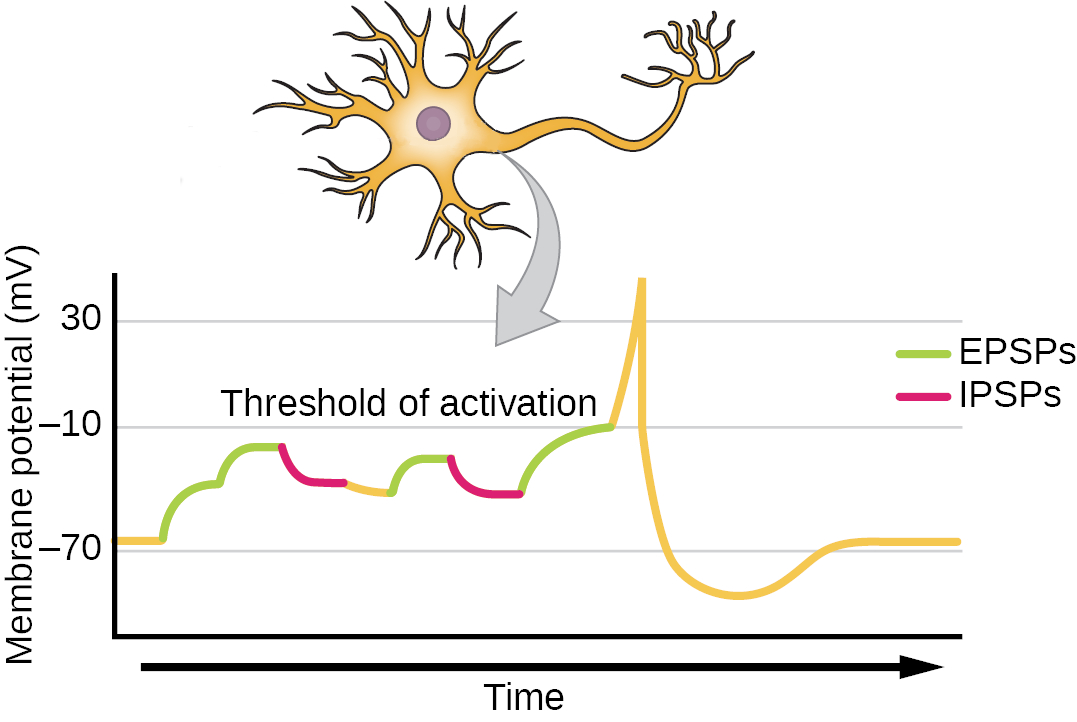
\includegraphics[height=150px]{gfx/Biological_Neuron_edited.jpg}
		\caption{Representation of a biological Neuron\\
			\cite{biology} edited}
		\label{fig:neuron1}
	\end{minipage}\hfill
	\begin{minipage}{0.45\textwidth}
		\centering
		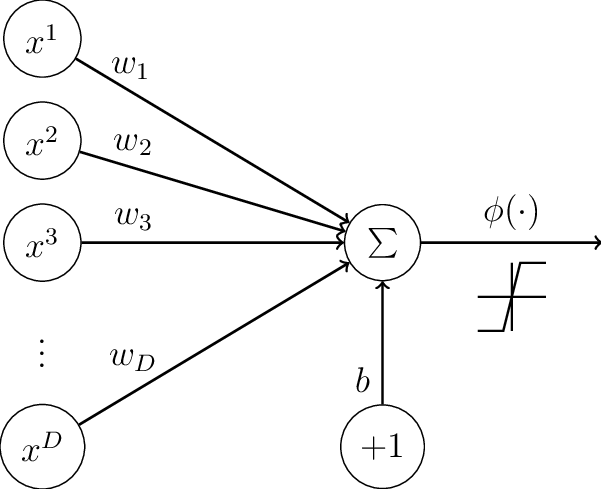
\includegraphics[height=150px]{gfx/Abstract_Neuron.png}
		\caption{Abstraction of a Neuron\\
			\cite{abstract_neuron}}
		\label{fig:neuron2}
	\end{minipage}
\end{figure}

\subsection{Data}
In addition to this model a numerical representation of any utilized data is also needed. A single data point is represented as a collection of inputs. Generally two descriptions can be distinguished:
\begin{itemize}
	\item \textbf{One-Hot-Encoding :}\\
	For each form the data point can assume a single input is modelled. Said input is activated if it fully represents the data otherwise it is not.\\
	Example:\\
	If a vocabulary of size $n$ is given its $m$-th word can be described as a vector with $n$ entries where only the $m$-th entry is non-zero.
	\item \textbf{Embedding :}\\
	If the data point can be described through features it can be though of as being embedded in a lower-dimensional more expressive space comparable to one-hot-encoding. An important advantage of this description is the resulting continuity of the input-space.\\
	Example: \\
	A sound could be described through its volume, pitch and duration
\end{itemize} 

\textbf{TODO: multidimensionality}

\subsection{Layers}
As an individual neuron is too simple to model any complex relations between inputs and outputs the next step is to aggregate multiple neurons. At the core of neural networks is the idea to collect the signal many different neurons produce for a given input and reuse them as new features for another round of neurons. Such a collection is called a \textbf{layer} and especially a \textbf{hidden layer} if neither its inputs were original data nor are its outputs the final activations. \footnote{
	This hierarchy of abstracts features is essential to the descriptive abilities of neural network. As such any sensible function between input and output can be approximated up to arbitrary precision by a network with at least one hidden layer. \cite{universal}
	}\\
A layer is defined by the structure of connections it prescribes. The layers used in this thesis consist of:

\begin{itemize}
	\item \textbf{Input :}\\
	The numeric representation of data points can be thought of activations a input-layer produces. In applications this layer is commonly used to describe assumptions on the data-points.  \\
	\item \textbf{Fully-Connected | Dense :}\\
	Every neuron of the layer is connected to every input.\\
	\item \textbf{Convolution :}\\
	Every neuron is only connected to a small neighbourhood of features.\\
	The Parameters are: neighbourhood size, amount of considered neighbourhoods and definition of behaviour at the edges of data points.\\
	Example:...\\
	\item \textbf{Pooling :}\\
	Not a conventional trainable layer but rather a data-processing-step between other layers. Reduces the number of features by condensing a small neighbourhood into a single feature.\\
	\item \textbf{Flatten :}\\  
	Not a conventional trainable layer but rather a data-processing-step between other layers. Collapses features from multiple dimensions into a single one.\\
\end{itemize}

\subsection{Architectures}
The collection of layers used for a given task is called an \textbf{architecture}. As multiple architectures are discussed throughout this work a clear system to note them is fundamental. Any architecture description first declares all default assumptions on its layers. Afterwards a list of layers follows defining the type of said layers, their hyper-parameters and especially the dimensionality of their outputs. Additionally and in interest of compatibility the following notation while be close to the functional Keras-API utilized throughout the associated source code.\\
The following two examples are meant to illustrate the notation:

\subsection*{1}
\begin{figure}[h]
	\centering
	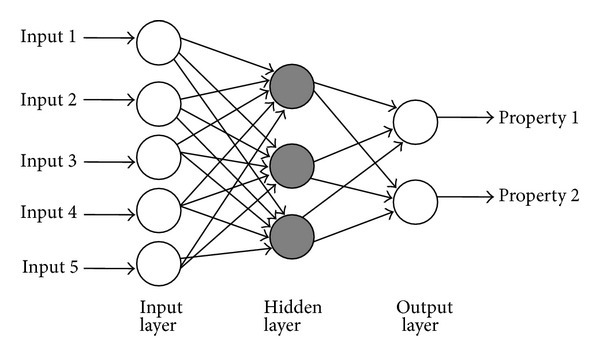
\includegraphics[height=200px]{gfx/Dense_FFNetwork.jpg}
	\caption{Architecture of a small fully-connected network\\
		\cite{dense_network}}
	\label{fig:FFNetwork}
\end{figure}
\begin{tabularx}{\textwidth}[!h]{X X X}
	\multicolumn{1}{c}{\textbf{Simple-FCN | \ref{fig:FFNetwork}}}\\
	\\
	\hline
	\endhead
	\textbf{Defaults} & Dense: activation & rectified linear unit\\
	\hline
	\textbf{Input} & output dimension & 5\\
	[8pt]
	\textbf{Dense} & output dimension & 3\\
	[8pt]
	\textbf{Dense} & output dimension & 2\\
	& activation & softmax\\
	\hline
\end{tabularx}

\newpage

\subsection*{2}

\begin{figure}[h]
	\centering
	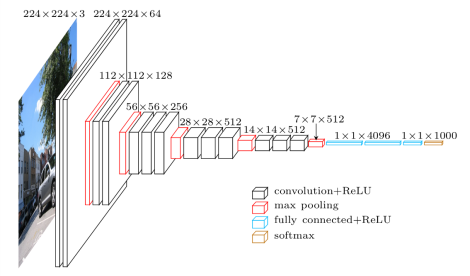
\includegraphics[height=200px]{gfx/vgg16.png}
	\caption{Macroarchitecture of VGG16\\
		\cite{VGG16}}
	\label{fig:VGG16}
\end{figure}


\begin{tabularx}{\textwidth}{X X X}
	\multicolumn{1}{c}{\textbf{VGG-16 | \ref{fig:VGG16}}}\\
	\\
	\hline
	\endhead
	\textbf{Defaults} & Convolution: kernel size & [3,3]\\
	& Convolution: stride & [1,1]\\
	& Convolution: paddig & same dimension\\
	& & zero padding\\
	& Softmax: kernel size & [2,2]\\
	& Softmax: stride & [1,1]\\
	\hline
	\textbf{Input} & output dimension & [224,224|3]\\
	[8pt]
	2x \textbf{Convolution} & output dimension & [224,224|64]\\
	[8pt]
	\textbf{Softmax} & output dimension & [112,112|64]\\
	[8pt]
	2x \textbf{Convolution} & output dimension & [112,112|128]\\
	[8pt]
	\textbf{Softmax} & output dimension & [56,56|128]\\
	[8pt]
	3x \textbf{Convolution} & output dimension & [56,56|256]\\
	[8pt]
	\textbf{Softmax} & output dimension & [28,28|256]\\
	[8pt]
	3x \textbf{Convolution} & output dimension & [28,28|512]\\
	[8pt]
	\textbf{Softmax} & output dimension & [14,14|512]\\
	[8pt]
	3x \textbf{Convolution} & output dimension & [14,14|512]\\
	[8pt]
	\textbf{Softmax} & output dimension & [7,7|512]\\
	[8pt]
	\textbf{Flatten} & output dimension & 25.088\\
	[8pt]
	\textbf{Dense} & output dimension & 4096\\
	[8pt]
	\textbf{Dense} & output dimension & 4096\\
	[8pt]
	\textbf{Dense} & output dimension & 1000\\
	& activation & softmax\\
	\hline
\end{tabularx}


\section{Pruning}
As the computational power of modern devices increases ever larger architectures become possible. While this allows for more precise models on any given data it is important to recall that pure representation is not the ultimate goal of most applications. Being more concrete, all tasks discussed in this work can be categorized as \textbf{supervised learning}, meaning they provide a collection of labelled data points and demand an extrapolation of the implicit labelling process, called \textbf{generalization}.
It is a well known phenomenon in the field of supervised learning\footnote{called \textbf{overfitting}} that generalization suffers from over-adaptation to the given data and that said over-adaptation tends to happen more easily in complex architectures.\\
On the other hand does massive parametrization not only enable us to approximate the labelling process\footnote{Which can be encoded as a function} more precisely but also to find such an approximation in a feasible way. \cite{Overparametrization}.\\
Pruning is a compromise in which a large model is fitted to a given data set and then truncated as much as possible while maintaining accuracy. 

\section{Preprocessing for Natural Language Processing}
In addition the previously mentioned treatment for any dataset there are additional preprocessing steps when handling text-inputs in natural language\footnote{The term \textbf{natural language} describes language written, spoken and otherwise used by humans in contrast to precisely defined languages used for communication between computation devices.}. The most important ones are \textbf{tokenization}, the separation of a text into words and/or sentences, and \textbf{stopword removal}, the removal of little to no syntactic or semantic importance.\\
As the former is almost always necessary to even quantify the numeric representation of the datapoints most frameworks provide datasets already preprocessed in such a manner.\\
The later is a canonical inclusion into any natural-language-processing data-flow but also is generally not preemptively applied to dataset.